%% This file was auto-generated by IPython, do NOT edit
%% Conversion from the original notebook file:
%% 05_Parallel_Computing.ipynb
%%
\documentclass[11pt,english]{article}

%% This is the automatic preamble used by IPython.  Note that it does *not*
%% include a documentclass declaration, that is added at runtime to the overall
%% document.

\usepackage{amsmath}
\usepackage{amssymb}
\usepackage{graphicx}
\usepackage{ucs}
\usepackage[utf8x]{inputenc}

% needed for markdown enumerations to work
\usepackage{enumerate}

% Slightly bigger margins than the latex defaults
\usepackage{geometry}
\geometry{verbose,tmargin=3cm,bmargin=3cm,lmargin=2.5cm,rmargin=2.5cm}

% Define a few colors for use in code, links and cell shading
\usepackage{color}
\definecolor{orange}{cmyk}{0,0.4,0.8,0.2}
\definecolor{darkorange}{rgb}{.71,0.21,0.01}
\definecolor{darkgreen}{rgb}{.12,.54,.11}
\definecolor{myteal}{rgb}{.26, .44, .56}
\definecolor{gray}{gray}{0.45}
\definecolor{lightgray}{gray}{.95}
\definecolor{mediumgray}{gray}{.8}
\definecolor{inputbackground}{rgb}{.95, .95, .85}
\definecolor{outputbackground}{rgb}{.95, .95, .95}
\definecolor{traceback}{rgb}{1, .95, .95}

% Framed environments for code cells (inputs, outputs, errors, ...).  The
% various uses of \unskip (or not) at the end were fine-tuned by hand, so don't
% randomly change them unless you're sure of the effect it will have.
\usepackage{framed}

% remove extraneous vertical space in boxes
\setlength\fboxsep{0pt}

% codecell is the whole input+output set of blocks that a Code cell can
% generate.

% TODO: unfortunately, it seems that using a framed codecell environment breaks
% the ability of the frames inside of it to be broken across pages.  This
% causes at least the problem of having lots of empty space at the bottom of
% pages as new frames are moved to the next page, and if a single frame is too
% long to fit on a page, will completely stop latex from compiling the
% document.  So unless we figure out a solution to this, we'll have to instead
% leave the codecell env. as empty.  I'm keeping the original codecell
% definition here (a thin vertical bar) for reference, in case we find a
% solution to the page break issue.

%% \newenvironment{codecell}{%
%%     \def\FrameCommand{\color{mediumgray} \vrule width 1pt \hspace{5pt}}%
%%    \MakeFramed{\vspace{-0.5em}}}
%%  {\unskip\endMakeFramed}

% For now, make this a no-op...
\newenvironment{codecell}{}

 \newenvironment{codeinput}{%
   \def\FrameCommand{\colorbox{inputbackground}}%
   \MakeFramed{\advance\hsize-\width \FrameRestore}}
 {\unskip\endMakeFramed}

\newenvironment{codeoutput}{%
   \def\FrameCommand{\colorbox{outputbackground}}%
   \vspace{-1.4em}
   \MakeFramed{\advance\hsize-\width \FrameRestore}}
 {\unskip\medskip\endMakeFramed}

\newenvironment{traceback}{%
   \def\FrameCommand{\colorbox{traceback}}%
   \MakeFramed{\advance\hsize-\width \FrameRestore}}
 {\endMakeFramed}

% Use and configure listings package for nicely formatted code
\usepackage{listingsutf8}
\lstset{
  language=python,
  inputencoding=utf8x,
  extendedchars=\true,
  aboveskip=\smallskipamount,
  belowskip=\smallskipamount,
  xleftmargin=2mm,
  breaklines=true,
  basicstyle=\small \ttfamily,
  showstringspaces=false,
  keywordstyle=\color{blue}\bfseries,
  commentstyle=\color{myteal},
  stringstyle=\color{darkgreen},
  identifierstyle=\color{darkorange},
  columns=fullflexible,  % tighter character kerning, like verb
}

% The hyperref package gives us a pdf with properly built
% internal navigation ('pdf bookmarks' for the table of contents,
% internal cross-reference links, web links for URLs, etc.)
\usepackage{hyperref}
\hypersetup{
  breaklinks=true,  % so long urls are correctly broken across lines
  colorlinks=true,
  urlcolor=blue,
  linkcolor=darkorange,
  citecolor=darkgreen,
  }

% hardcode size of all verbatim environments to be a bit smaller
\makeatletter 
\g@addto@macro\@verbatim\small\topsep=0.5em\partopsep=0pt
\makeatother 

% Prevent overflowing lines due to urls and other hard-to-break entities.
\sloppy

\begin{document}
\begin{center}
{\bf \Large Parallel Computing with IPython}

{\bf \large Python in HPC}

{\bf TACC Training, Oct. 15, 2012}
\end{center}

\noindent Presenters:

\noindent {\bf Andy R. Terrel, PhD}\\
Texas Advanced Computing Center\\
University of Texas at Austin\\

\noindent {\bf Yaakoub El Khamra}\\
Texas Advanced Computing Center\\
University of Texas at Austin\\

\href{http://creativecommons.org/licenses/by/3.0/deed.en\_US}{\includegraphics{figures/creative_commons_logo.png}}\\

\noindent Python in HPC Tutorial by Terrel, and El Khamra is licensed
under a Creative Commons Attribution 3.0 Unported License. \\[2em]

\href{http://www.tacc.utexas.edu}{\includegraphics[scale=0.8]{figures/TACC_logo.png}} \qquad

\newpage

\newpage

\subsection{Interacting with the Tutorial Slides}

This tutorial is an interactive worksheet designed to encourage you to
try out the lessons during the demonstration. If you are looking at the
pdf version, we encourage you to download the updated version (see
previous slide) and try the interactive version.

To run the interactive version, you need a good Python environment
including:

\begin{itemize}
\item
  IPython version \textgreater{}= 13.0
\item
  Numpy version \textgreater{}= 1.5
\item
  Scipy
\item
  Matplotlib
\end{itemize}

Move to the directory containing the tarball and execute:

\begin{verbatim}
$ ipython notebook --pylab=inline
\end{verbatim}

We heartily endorse the
\href{https://store.continuum.io/cshop/anaconda}{Anaconda distribution}
and the \href{http://www.enthought.com/products/epd\_free.php}{Free
Enthought Python Distribution}.

\newpage

\subsection{Presentation mode}

 The slide show mode is only supported by an IPython development branch
version. To get it I recommend cloning from the official branch, adding
Matthias Carreau's remote, fetching and using his branch
slideshow\_extension2. Here are the commands:

\begin{verbatim}
git clone git://github.com/ipython/ipython.git # Official clone
cd ipython
git remote add carreau git://github.com/Carreau/ipython.git # Matthias' branch
git fetch carreau # Fetch the branches
git checkout carreau/slideshow_extension2 # Checkout the slideshow extension
python setup.py develop # Install the development version
ipython notebook # Check out the slideshows.
\end{verbatim}



\newpage

\section{Architecture Overview}

\begin{figure}[htbp]
\centering
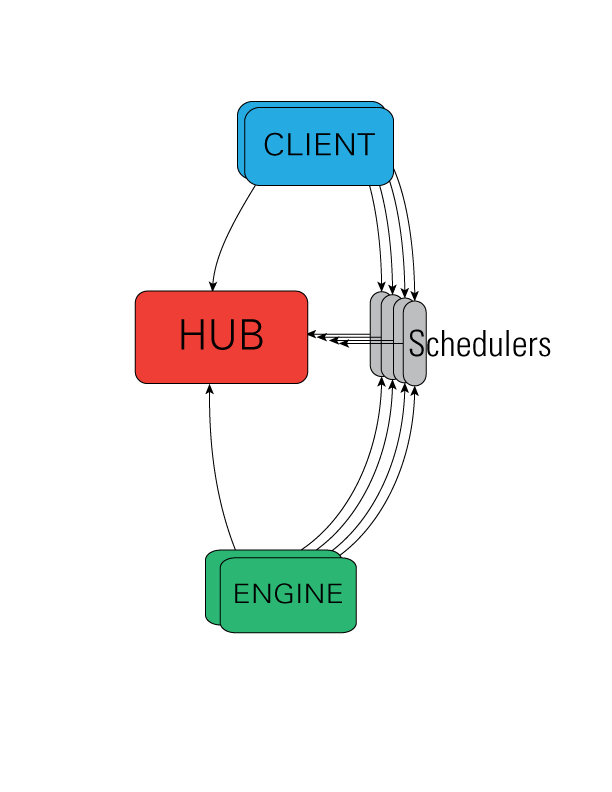
\includegraphics{figures/wideView.png}
\caption{Architecture}
\end{figure}

The IPython architecture consists of four components:

\begin{itemize}
\item
  The IPython engine
\item
  The IPython hub
\item
  The IPython schedulers
\item
  The controller client
\end{itemize}

\newpage

\subsection{The Engine(s)}

The IPython engine is a Python instance that takes Python commands over
a network connection. Eventually, the IPython engine will be a full
IPython interpreter, but for now, it is a regular Python interpreter.
The engine can also handle incoming and outgoing Python objects sent
over a network connection. When multiple engines are started, parallel
and distributed computing becomes possible. An important feature of an
IPython engine is that it blocks while user code is being executed.

\newpage

\subsection{The Controller}

The IPython controller processes provide an interface for working with a
set of engines. At a general level, the controller is a collection of
processes to which IPython engines and clients can connect. The
controller is composed of a Hub and a collection of Schedulers. These
Schedulers are typically run in separate processes but on the same
machine as the Hub, but can be run anywhere from local threads or on
remote machines.

The controller also provides a single point of contact for users who
wish to utilize the engines connected to the controller. There are
different ways of working with a controller. In IPython, all of these
models are implemented via the View.apply() method, after constructing
View objects to represent subsets of engines. The two primary models for
interacting with engines are:

\begin{itemize}
\item
  Direct interface, where engines are addressed explicitly.
\item
  LoadBalanced interface, where the Scheduler is trusted with assigning
  work to appropriate engines.
\end{itemize}

Advanced users can readily extend the View models to enable other styles
of parallelism.

\newpage

\subsection{The Hub}

The center of an IPython cluster is the Hub. This is the process that
keeps track of engine connections, schedulers, clients, as well as all
task requests and results. The primary role of the Hub is to facilitate
queries of the cluster state, and minimize the necessary information
required to establish the many connections involved in connecting new
clients and engines.

\newpage

\subsection{The Scheduler(s)}

All actions that can be performed on the engine go through a Scheduler.
While the engines themselves block when user code is run, the schedulers
hide that from the user to provide a fully asynchronous interface to a
set of engines.

\newpage

\subsection{Starting the IPython Controller and Engines}

 We already did this. We used: !ipcluster start --engines=MPI --n 4 to
launch 4 MPI engines.

There are two ways to start the controller and engines:

\begin{itemize}
\item
  In an automated manner using the ipcluster command (possibly with a
  profile)
\item
  In a more manual way using the ipcontroller and ipengine commands
\end{itemize}

Use ipcluster (with a profile) whenever possible. The profile will live
in IPYTHONDIR/profile\_\textless{} profile name \textgreater{}/ (usually
\$HOME/.ipython\ldots{}) and that directory needs to be accessible to
controller and engines.

ipcluster supports:

\begin{itemize}
\item
  all local: controller and engines are on the same node (we are doing
  this)
\item
  engines are started with mpiexec (we are also doing this)
\item
  engines are started with a batch system (PBS/SGE)
\item
  controller is on the localhost, the engines are started remotely with
  ssh
\end{itemize}

For more information on how to configure a profile for ipcluster, please
refer to the
\href{http://ipython.org/ipython-doc/dev/parallel/parallel\_process.html}{IPython
documentation}

\newpage

\subsection{The Client and Views}

There is one primary object, the Client, for connecting to a cluster.
For each execution model, there is a corresponding View. These views
allow users to interact with a set of engines through the interface.
There are two default views:

\begin{itemize}
\item
  DirectView class for explicit addressing
\item
  LoadBalanceView class for destination-agnostic scheduling
\end{itemize}

\newpage

\subsection{The DirectView}

 The direct, or multiengine, interface represents one possible way of
working with a set of IPython engines. The basic idea behind the
multiengine interface is that the capabilities of each engine are
directly and explicitly exposed to the user. Thus, in the multiengine
interface, each engine is given an id that is used to identify the
engine and give it work to do. This interface is very intuitive and is
designed with interactive usage in mind, and is the best place for new
users of IPython to begin.

\begin{codecell}
\begin{codeinput}
\begin{lstlisting}
# import the parallel module and create a Client instance
from IPython.parallel import Client
rc = Client()
# check the id's of the engines
print rc.ids
# Create a DirectView object that will use all of the available engines
direct_view = rc[:]

\end{lstlisting}
\end{codeinput}
\begin{codeoutput}
\begin{verbatim}
[0, 1, 2, 3]
\end{verbatim}
\end{codeoutput}
\end{codecell}
\newpage

\subsection{The map() function}

Python's builtin map() functions allows a function to be applied to a
sequence element-by-element (and is thus trivial to parallelize). The
DirectView`s version of map() does not do dynamic load balancing

\begin{codecell}
\begin{codeinput}
\begin{lstlisting}
# serial version run on the controller
serial_result = map(lambda x:x**10, range(32))
# parallel version run on the engines
parallel_result = direct_view.map_sync(lambda x: x**10, range(32))
# make sure they are equal
serial_result==parallel_result
\end{lstlisting}
\end{codeinput}
\begin{codeoutput}
\begin{verbatim}
True
\end{verbatim}
\end{codeoutput}
\end{codecell}
\newpage

\subsection{Remote Function Decorators}

Remote functions are just like normal functions, but when they are
called, they execute on one or more engines, rather than locally.
IPython provides two decorators:

\begin{codecell}
\begin{codeinput}
\begin{lstlisting}
@direct_view.remote(block=True)
def getpid():
    import os
    return os.getpid()
\end{lstlisting}
\end{codeinput}
\end{codecell}
\begin{codecell}
\begin{codeinput}
\begin{lstlisting}
getpid()
\end{lstlisting}
\end{codeinput}
\begin{codeoutput}
\begin{verbatim}
[8627, 8630, 8629, 8628]
\end{verbatim}
\end{codeoutput}
\end{codecell}
The @parallel decorator creates parallel functions, that break up an
element-wise operations and distribute them, reconstructing the result.

\begin{codecell}
\begin{codeinput}
\begin{lstlisting}
import numpy as np
A = np.random.random((64,48))

@direct_view.parallel(block=True)
def pmul(A,B):
    return A*B

C_local = A*A

C_remote = pmul(A,A)

(C_local == C_remote).all()
\end{lstlisting}
\end{codeinput}
\begin{codeoutput}
\begin{verbatim}
True
\end{verbatim}
\end{codeoutput}
\end{codecell}
Calling a @parallel function does not correspond to map. It is used for
splitting element-wise operations that operate on a sequence or array.
For map behavior, parallel functions do have a map method.

\newpage

\subsection{Calling Python functions}

The most basic type of operation that can be performed on the engines is
to execute Python code or call Python functions. Executing Python code
can be done in blocking or non-blocking mode (non-blocking is default)
using the View.execute() method, and calling functions can be done via
the View.apply() method.

\begin{codecell}
\begin{codeinput}
\begin{lstlisting}
# Setup a blocking view
blocking_direct_view = rc[:]
blocking_direct_view.block = True

# Set the values of a and b on all engines
blocking_direct_view['a'] = 10
blocking_direct_view['b'] = 12

# Apply a function
blocking_direct_view.apply(lambda x: a+b+x, 5)
\end{lstlisting}
\end{codeinput}
\begin{codeoutput}
\begin{verbatim}
[27, 27, 27, 27]
\end{verbatim}
\end{codeoutput}
\end{codecell}
Alternatively you can execute Python commands as strings on specific
engines

\begin{codecell}
\begin{codeinput}
\begin{lstlisting}
# execute on 0 and 2
rc[::2].execute('c=a+b')
# execute on 1 and 3
rc[1::2].execute('c=a-b')
# retrieve c from the engines
blocking_direct_view['c']
\end{lstlisting}
\end{codeinput}
\begin{codeoutput}
\begin{verbatim}
[22, -2, 22, -2]
\end{verbatim}
\end{codeoutput}
\end{codecell}
In non-blocking mode, apply() submits the command to the engine and
returns immediately with a AsyncResult object. To retrieve the result
you can use the get() method from the
\href{http://ipython.org/ipython-doc/dev/parallel/asyncresult.html\#parallel-asyncresult}{AsyncResult}
object. The advantage of using non-blocking execution is that you can
submit commands that possibly take a long time to execute without
blocking the controller (particularly useful in interactive sessions).

\begin{codecell}
\begin{codeinput}
\begin{lstlisting}
non_blocking_direct_view = rc[:]
non_blocking_direct_view.block = False

# create a dummy wait function
def wait(t):
    import time
    tic = time.time()
    time.sleep(t)
    return time.time()-tic

# in non-blocking mode
ar = non_blocking_direct_view.apply_async(wait,2)
# now block for the result
ar.get()
                
\end{lstlisting}
\end{codeinput}
\begin{codeoutput}
\begin{verbatim}
[2.0009918212890625, 2.000959873199463, 2.001322031021118, 2.00095796585083]
\end{verbatim}
\end{codeoutput}
\end{codecell}
\begin{codecell}
\begin{codeinput}
\begin{lstlisting}
ar = non_blocking_direct_view.apply_async(wait,10)

# poll to see if the result is ready
ar.ready()
\end{lstlisting}
\end{codeinput}
\begin{codeoutput}
\begin{verbatim}
False
\end{verbatim}
\end{codeoutput}
\end{codecell}
\begin{codecell}
\begin{codeinput}
\begin{lstlisting}
# Ask for the result but wait for a maximum of 1 second:
ar.get(1)
\end{lstlisting}
\end{codeinput}
\begin{codeoutput}
\begin{verbatim}
[10.00077199935913, 10.000739097595215, 10.00072193145752, 10.0003080368042]
\end{verbatim}
\end{codeoutput}
\end{codecell}
\newpage

\subsection{Moving Objects around}

Use push() and pull() to send and get objects from engines

\begin{codecell}
\begin{codeinput}
\begin{lstlisting}
blocking_direct_view.push(dict(a=1.03234,b=3453))
\end{lstlisting}
\end{codeinput}
\begin{codeoutput}
\begin{verbatim}
[None, None, None, None]
\end{verbatim}
\end{codeoutput}
\end{codecell}
\begin{codecell}
\begin{codeinput}
\begin{lstlisting}
blocking_direct_view.pull('a')
\end{lstlisting}
\end{codeinput}
\begin{codeoutput}
\begin{verbatim}
[1.03234, 1.03234, 1.03234, 1.03234]
\end{verbatim}
\end{codeoutput}
\end{codecell}
\begin{codecell}
\begin{codeinput}
\begin{lstlisting}
blocking_direct_view.pull('b', targets=0)
\end{lstlisting}
\end{codeinput}
\begin{codeoutput}
\begin{verbatim}
3453
\end{verbatim}
\end{codeoutput}
\end{codecell}
\begin{codecell}
\begin{codeinput}
\begin{lstlisting}
blocking_direct_view.pull(('a','b'))
\end{lstlisting}
\end{codeinput}
\begin{codeoutput}
\begin{verbatim}
[[1.03234, 3453], [1.03234, 3453], [1.03234, 3453], [1.03234, 3453]]
\end{verbatim}
\end{codeoutput}
\end{codecell}
\begin{codecell}
\begin{codeinput}
\begin{lstlisting}
blocking_direct_view.push(dict(c='speed'))
\end{lstlisting}
\end{codeinput}
\begin{codeoutput}
\begin{verbatim}
[None, None, None, None]
\end{verbatim}
\end{codeoutput}
\end{codecell}
In non-blocking mode, push() and pull() return AsyncResult objects

\begin{codecell}
\begin{codeinput}
\begin{lstlisting}
ar = non_blocking_direct_view.pull('a')
ar.get()
\end{lstlisting}
\end{codeinput}
\begin{codeoutput}
\begin{verbatim}
[1.03234, 1.03234, 1.03234, 1.03234]
\end{verbatim}
\end{codeoutput}
\end{codecell}
\newpage

\subsection{Parallel Magic Commands}

IPython has a few magic commands that make executing Python commands in
parallel a lot more pleasant. The magics will be automatically available
when we create a client:

rc = parallel.Client()

\begin{codecell}
\begin{codeinput}
\begin{lstlisting}
# Import numpy everywhere, including controller
with rc[:].sync_imports():
    import numpy
\end{lstlisting}
\end{codeinput}
\begin{codeoutput}
\begin{verbatim}
importing numpy on engine(s)
\end{verbatim}
\end{codeoutput}
\end{codecell}
The \%px magic executes a single Python command on the engines specified
by the targets attribute of the DirectView instance:

\begin{codecell}
\begin{codeinput}
\begin{lstlisting}
%px a = numpy.random.rand(2,2)
# to see the result:
%px print a
\end{lstlisting}
\end{codeinput}
\begin{codeoutput}
\begin{verbatim}
[stdout:0] 
[[ 0.75807677  0.55011869]
 [ 0.06067355  0.23753211]]
[stdout:1] 
[[ 0.31290721  0.70553545]
 [ 0.25818139  0.03566729]]
[stdout:2] 
[[ 0.39323519  0.98505994]
 [ 0.64079498  0.3318084 ]]
[stdout:3] 
[[ 0.44615847  0.66901976]
 [ 0.80198817  0.74741971]]
\end{verbatim}
\end{codeoutput}
\end{codecell}


\begin{codecell}
\begin{codeinput}
\begin{lstlisting}
%%px --targets ::2
print "I am even"
\end{lstlisting}
\end{codeinput}
\begin{codeoutput}
\begin{verbatim}
[stdout:0] I am even
[stdout:2] I am even
\end{verbatim}
\end{codeoutput}
\end{codecell}
\begin{codecell}
\begin{codeinput}
\begin{lstlisting}
%%px --targets 1
print "I am number 1"
\end{lstlisting}
\end{codeinput}
\begin{codeoutput}
\begin{verbatim}
I am number 1
\end{verbatim}
\end{codeoutput}
\end{codecell}
Important magic notes:

\begin{itemize}
\item
  If you are using \%px in non-blocking mode, you won't get output. You
  can use \%pxresult to display the outputs of the latest command, just
  as is done when \%px is blocking
\item
  The \%autopx magic switches to a mode where everything you type is
  executed on the engines until you do \%autopx again
\item
  You can change the blocking and targets attributes of the active view
  with \%pxconfig
\item
  You can change the active view by calling the activate method on any
  view
\end{itemize}

\end{document}
